\begin{starred}
    \chapter{\texorpdfstring{视图\footnote{本章为选学内容。}}{视图(选学)}}
\end{starred}

在房屋建筑、水利施工、零件附造、机器装配检修中,都是以图纸为依据的。搞技术革新、搞自动化更是离不开图纸。
这是因为只用文字语言,很难清楚地表达出一个机器的结构、形状和大小,所以图纸是一种重要的技术文件。
为了学会看图纸的基本技能,在这一章里,我们介绍视图的一些初步知识。

\subsection{视图}\label{subsec:czjh2-8-1}

\begin{wrapfigure}[7]{r}{5cm}
    \centering
    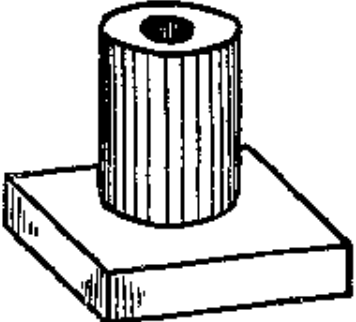
\includegraphics[width=3cm]{../pic/czjh2-ch8-01.png}
    \caption{}\label{fig:czjh2-8-1}
\end{wrapfigure}

图 \ref{fig:czjh2-8-1} 是工厂里常见的一个机械零件的直观图,这种图虽富有立体感,
但不能准确地表示出物体各部分的真实形状和内部结构。
如长方形变成了平行四边形,圆变成了椭圆,并且看不清圆孔的深度,图形各部分尺寸也有了变化。
因此,一般不根据直观图来加工零件,而把它作为辅助图来使用。

为了准确地表示物体的实际形状和尺寸大小,在生产中主要采用视图,视图是用投影原理画出来的。

\subsubsection{投影}

投影现象广泛地存在于自然界和日常生活中,如在灯光下,将两手交叉握紧,
墙上就会出现象动物头部的影子(图 \ref{fig:czjh2-8-2}),墙壁是投影面,光线是投射线,
影子就是手在墙上的投影,由于灯光的光线可以看作是从一点发出的,
我们称这种投影为\zhongdian{中心投影}。

又如在阳光下,树的影子是树在地面上的投影,地面是投影面,光线是投射线。
由于太阳的光线可看作是平行的,这时,我们称这种投影为\zhongdian{平行投影}。

\begin{figure}[htbp]
    \centering
    \begin{minipage}[b]{7cm}
        \centering
        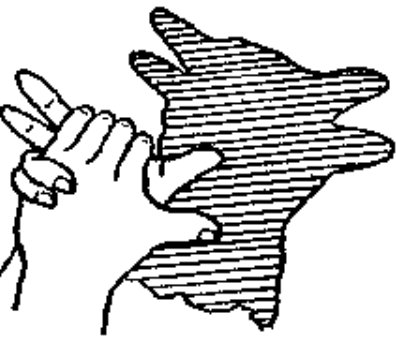
\includegraphics[width=4cm]{../pic/czjh2-ch8-02.png}
        \caption{}\label{fig:czjh2-8-2}
    \end{minipage}
    \begin{minipage}[b]{7cm}
        \centering
        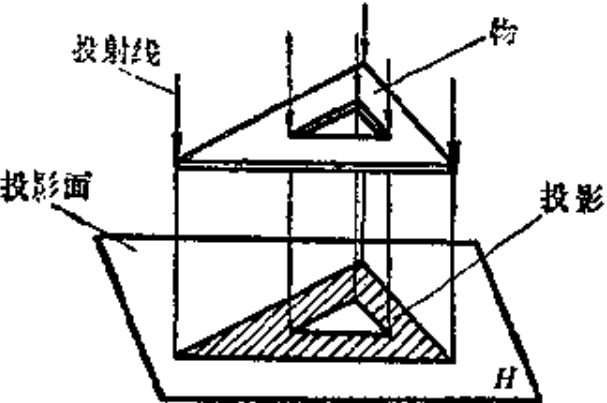
\includegraphics[width=6cm]{../pic/czjh2-ch8-03.png}
        \caption{}\label{fig:czjh2-8-3}
    \end{minipage}
\end{figure}

在平行投影中,如果投射线垂直于投影面,那么这种投影就称为\zhongdian{正投影}。
如图 \ref{fig:czjh2-8-3},一块三角板对于投影面 $H$ 平放着,光线垂直于投影面,
这时三角板的投影与它本身的形状、大小都一样。

我们看出,正投影能够反映物体的真实形状和大小。
因此,在工程技术上使用的图纸,多采用正投影方法绘制。


\subsubsection{正投影的规律}

(1)线段的正投影

如图 \ref{fig:czjh2-8-4},
点 $A$ 的投影为点 $A'$,记作 $A \to A'$,
点 $B$ 的投影为点 $B'$,记作 $B \to B'$;
线段 $AB$ 的投影为线段 $A'B'$,记作 $AB \to A'B'$。

\begin{figure}[htbp]
    \centering
    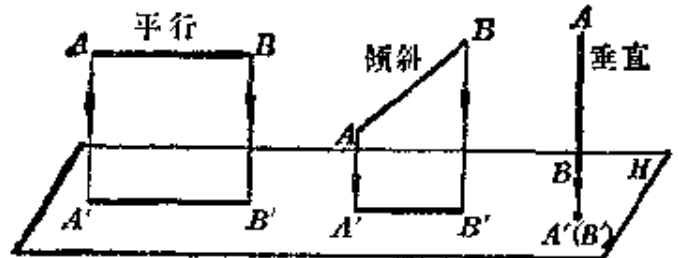
\includegraphics[width=8cm]{../pic/czjh2-ch8-04.png}
    \caption{}\label{fig:czjh2-8-4}
\end{figure}

当 $AB$ 平行于投影面 $H$ 时,$A'B' = AB$,“长不变”;

当 $AB$ 倾斜于投影面 $H$ 时,$A'B' < AB$,“长缩短”;

当 $AB$ 垂直于投影面 $H$ 时,$A' \equiv B'$\footnotemark,“成一点”。
\footnotetext{$A' \equiv B'$ 表示点 $A'$、$B'$ 重合,“$\equiv$” 在这里是重合记号。}

由此得到线段的正投影规律:

\begin{center}
    \framebox{\zhongdian{平行长不变,倾斜长缩短,垂直成一点。}}
\end{center}


(2)平面形的正投影

如图 \ref{fig:czjh2-8-5},平面形 $P$ (即四边形 $ABCD$)在投影面 $H$ 上的投影为四边形 $A'B'C'D'$。

\begin{figure}[htbp]
    \centering
    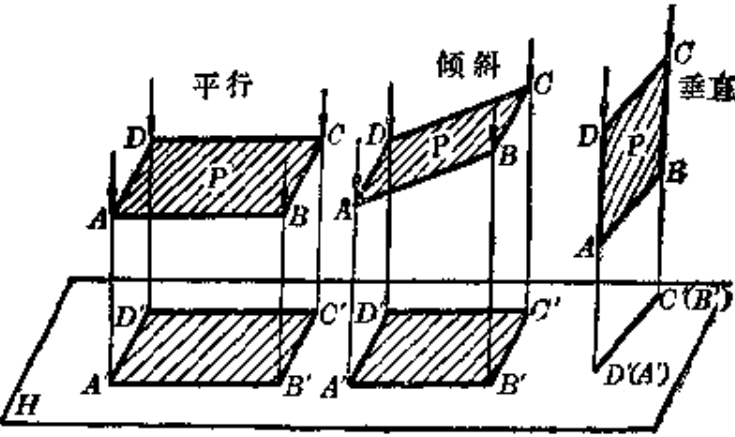
\includegraphics[width=8cm]{../pic/czjh2-ch8-05.png}
    \caption{}\label{fig:czjh2-8-5}
\end{figure}

$\because$ \quad $AB \to A'B'$, $BC \to B'C'$, $CD \to C'D'$, $DA \to D'A'$,

$\therefore$ \quad $\text{四边形} \; ABCD \to \text{四边形} \; A'B'C'D'$。

当图形 $P$ 平行于投影面 $H$ 时,$\text{四边形} \; ABCD \quandeng \text{四边形} \; A'B'C'D'$,“形状不变”;

当图形 $P$ 倾斜于投影面 $H$ 时,“形状改变”;

当图形 $P$ 垂直于投影面 $H$ 时,“成线段”。

由此得到平面形的正投影规律:

\begin{center}
    \framebox{\zhongdian{平行形不变,倾斜形改变,垂直成线段。}}
\end{center}


(3)几何体的正投影

一个正方体与投影面 $V$ 的相对位置如图 \ref{fig:czjh2-8-6} 所示,正方体有六个面:
面 $P$、$Q$、$R$ 和分别与它们相对的三个面。
根据平面形的正投影规律,我们可以得到这六个面的正投影。

因为面 $P$、$Q$ 及其相对的面都与投影面 $V$ 垂直,就有

面 $P \to A'B'$,面 $P$ 相对的面 $\to D'C'$;

面 $Q \to B'C'$,面 $Q$ 相对的面 $\to A'D'$;

面 $R$ 及其相对的面平行于投影面 $V$,就有

面 $R \to$ 正方形 $A'B'C'D'$,面 $R$ 相对的面 $\to$ 正方形 $A'B'C'D'$。

所以,正方体在投影面 $V$ 上的正投影是正方形 $A'B'C'D'$。

物体的正投影称为物体的\zhongdian{视图}。

物体的视图与物体对于投影面的位置有关,当正方体在如图 \ref{fig:czjh2-8-6} 中的位置吋,
它在投影面 $V$ 上的视图是一个正方形。而在其他位置时就不一定是正方形。


\begin{figure}[htbp]
    \centering
    \begin{minipage}[b]{7cm}
        \centering
        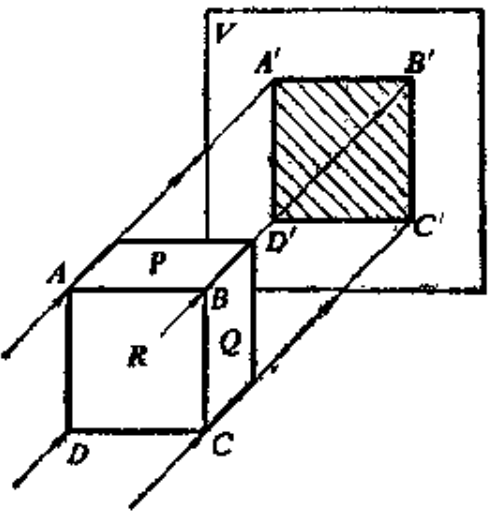
\includegraphics[width=5cm]{../pic/czjh2-ch8-06.png}
        \caption{}\label{fig:czjh2-8-6}
    \end{minipage}
    \begin{minipage}[b]{7cm}
        \centering
        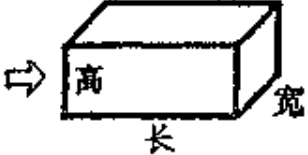
\includegraphics[width=4cm]{../pic/czjh2-ch8-subsec1-lx-03.png}
        \caption*{(第 3 题)}
    \end{minipage}
\end{figure}


\begin{lianxi}

\xiaoti{举出几个日常生活中的例子说明投影概念。}

\xiaoti{有一圆形木板,它的正投影一定是圆形吗?为什么?}

\xiaoti{已知长方体的长、宽、高分别为 3 cm、2 cm、1 cm,
    说出图中所示方向的视图,并用平面形的正投影规律加以说明。
}

\end{lianxi}


\subsection{二视图}\label{subsec:czjh2-8-2}

\subsubsection{二视图的概念}

当一些物体或零件比较复杂时,只用一个正投影图很难把它的形状特征表示清楚,
这时往往需要从不同的投射方向,把物体或零件投影到两个互相垂直的投影面上,用两个正投影图来表示它们。
\begin{figure}[htbp]
    \centering
    \begin{minipage}[b]{7cm}
        \centering
        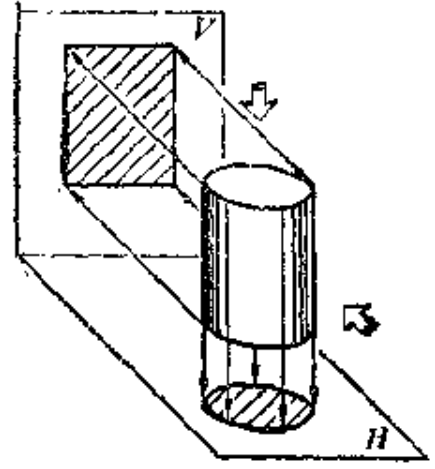
\includegraphics[width=4cm]{../pic/czjh2-ch8-07.png}
        \caption{}\label{fig:czjh2-8-7}
    \end{minipage}
    \begin{minipage}[b]{7cm}
        \centering
        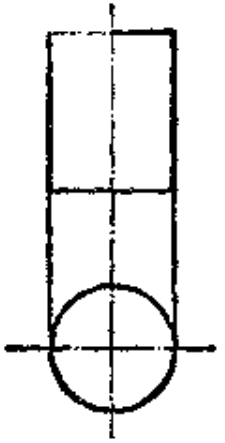
\includegraphics[width=2cm]{../pic/czjh2-ch8-08.png}
        \caption{}\label{fig:czjh2-8-8}
    \end{minipage}
\end{figure}
下面我们来看将一个圆柱放在互相垂直的两个投影面间进行正投影的情形。
如图 \ref{fig:czjh2-8-7} 所示,在正面投影面 $V$ 上的视图是一个矩形,长等于圆柱的直径,
高等于圆柱的高,在水平投影面 $H$ 上的视图是一个圆,它与圆柱的底是等圆。



将圆柱拿走,把水平投影面 $H$ 往下转 $90^\circ$,使投影面 $H$ 与 $V$ 在同一平面上,
我们就得到如图 \ref{fig:czjh2-8-8} 所示的图形。

在正面投影面 $V$ 上所得到的视图称为\zhongdian{主视图};

在水平投影面 $H$ 上所得到的视图称为\zhongdian{俯视图}。

主视图和俯视图统称为\zhongdian{二视图}。

画物体的二视图时,主视图画在上面,俯视图画在它的下面,而且两个视图要对正。
画对称形物体的视图时,要先画物体的对称轴线或中心线,用点划线表示。

现在我们以图 \ref{fig:czjh2-8-1} 中的零件上半部为例,研究这个空心圆柱的二视图。

空心圆柱的外形是圆柱,空心部分也是圆柱,所以它的俯视图是两个同心圆,它的主视图是两个矩形。
如图 \ref{fig:czjh2-8-9} 所示,圆柱的外形部分是看得见的,画粗实线;圆柱的空心部分是看不见的,画虚线。

\begin{figure}[htbp]
    \centering
    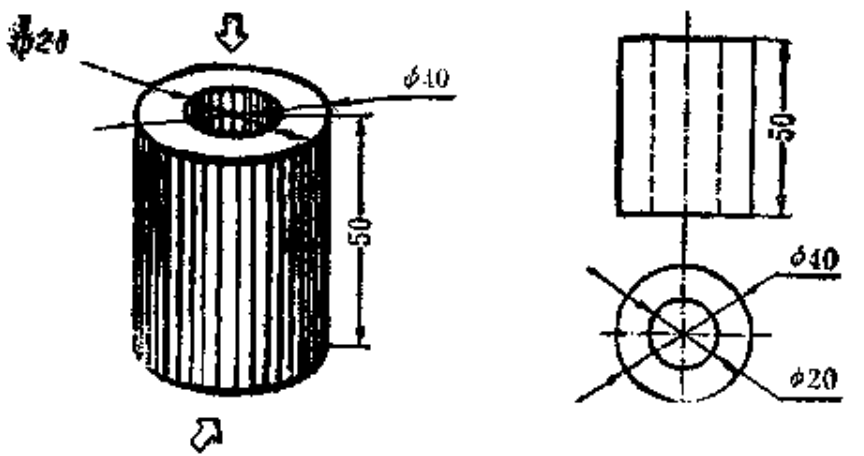
\includegraphics[width=8cm]{../pic/czjh2-ch8-09.png}
    \caption{}\label{fig:czjh2-8-9}
\end{figure}

在画视图时规定,\zhongdian{看得见部分的轮廓线画粗实线,看不见部分的轮廓线画虚线。}

每一个视图画好后,都要标注尺寸,这样便于加工。图纸上不具体注明尺寸单位的都是指 mm ,
如图 \ref{fig:czjh2-8-9},图中高 50 就是 50 mm, $\phi 40$ 就是直径为 40 mm。
图线的使用和尺寸的注法可参看本章\hyperref[sec:czjh2-8-fulu]{附录}。

二视图的画法规则可以概括为

\begin{center}
    \framebox{\zhongdian{上主下俯长对正,实线虚线要分清。}}
\end{center}


\subsubsection{二视图的画法}

以圆锥为例,如图 \ref{fig:czjh2-8-10}(a),它的二视图应该怎样画呢?
根据二视图的画法规则,圆锥的主视图是一个等腰三角形,俯视图是一个圆。
圆锥的二视图的具体画法如下:

\begin{figure}[htbp]
    \centering
    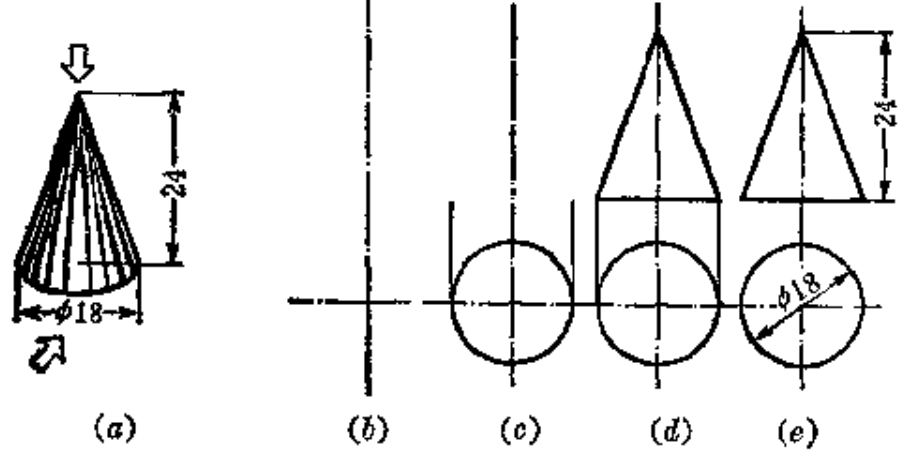
\includegraphics[width=9cm]{../pic/czjh2-ch8-10.png}
    \caption{}\label{fig:czjh2-8-10}
\end{figure}

(1)画出对称轴线 —— 点划线,如图 \ref{fig:czjh2-8-10}(b);

(2)画出俯视图,即画直径为 18 mm 的圆,如图 \ref{fig:czjh2-8-10}(c);

(3)根据主视图、俯视图上下长对正与已知圆锥的高等于 24 mm,画出等腰三角形,如图 \ref{fig:czjh2-8-10}(d);

(4)标注尺寸,擦去不必要的辅助线,如图 \ref{fig:czjh2-8-10}(e)。

再如画圆台的二视图,如图 \ref{fig:czjh2-8-11}(a),已知圆台上下两底的直径分别为 20 mm和 40 mm,高为 40 mm,
它的二视图的画法步骤与圆锥二视图的画法相同,具体画法如图 \ref{fig:czjh2-8-11}(b)、(c)、(d)、(e),由同学自己分析。

% \begin{figure}[htbp]
%     \centering
%     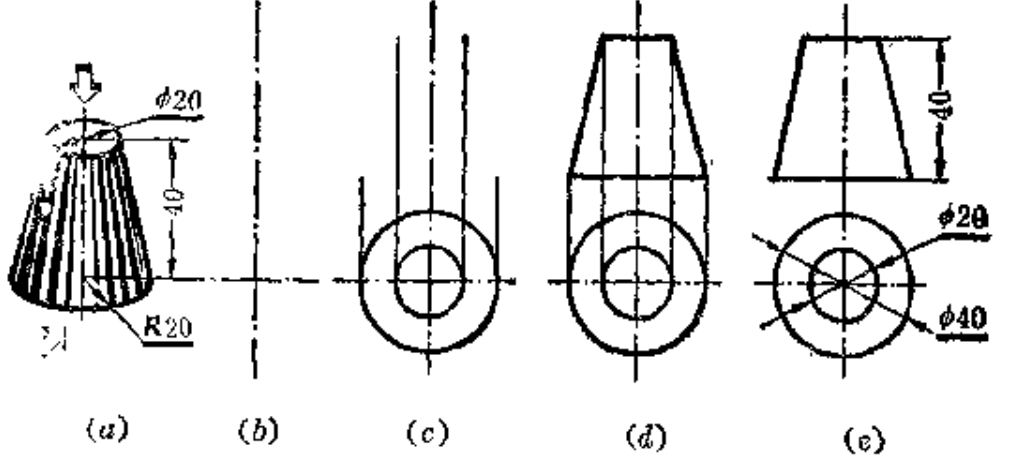
\includegraphics[width=9cm]{../pic/czjh2-ch8-11.png}
%     \caption{}\label{fig:czjh2-8-11}
% \end{figure}

画图时,可以根据实物的大小和其结构的复杂程度,用一定的比例尺进行放大或缩小。
加工零件时,以图上的尺寸数字为准。

\begin{figure}[htbp]
    \centering
    \begin{minipage}[b]{10cm}
        \centering
        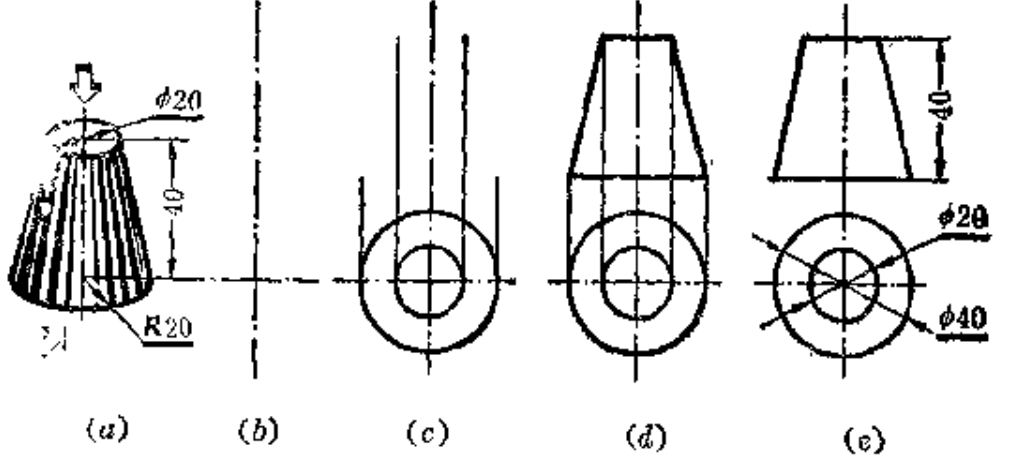
\includegraphics[width=9cm]{../pic/czjh2-ch8-11.png}
        \caption{}\label{fig:czjh2-8-11}
    \end{minipage}
    \begin{minipage}[b]{4cm}
        \centering
        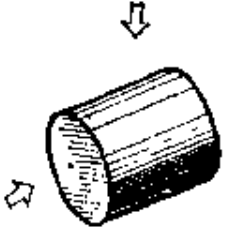
\includegraphics[width=3cm]{../pic/czjh2-ch8-subsec2-lx-01.png}
        \caption*{(第 1 题)}
    \end{minipage}
\end{figure}

\begin{lianxi}

\xiaoti{任何圆柱的主视图总是矩形,俯视图总是圆,这种说法对吗?如果圆柱按图中的放法,它的二视图是怎样的?}

\xiaoti{说出下列几何体的二视图。}

\begin{figure}[htbp]
    \centering
    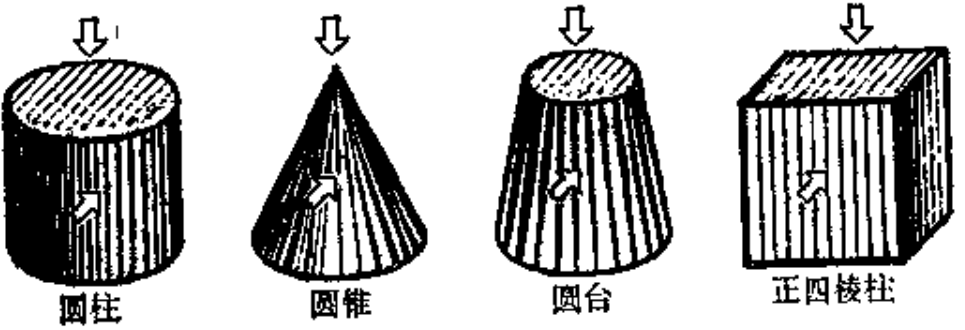
\includegraphics[width=9cm]{../pic/czjh2-ch8-subsec2-lx-02.png}
    \caption*{(第 2 题)}
\end{figure}

\xiaoti{下面是空心圆柱的二视图,哪个有错误?为什么错?}

\begin{figure}[htbp]
    \centering
    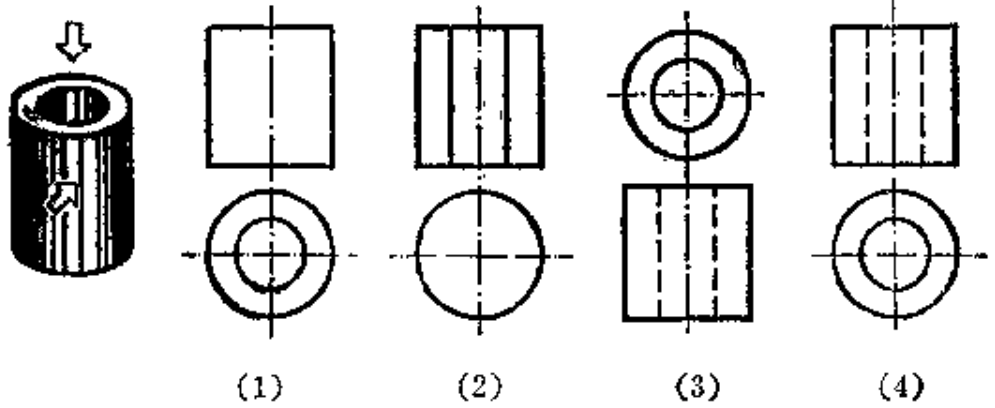
\includegraphics[width=9cm]{../pic/czjh2-ch8-subsec2-lx-03.png}
    \caption*{(第 3 题)}
\end{figure}

\end{lianxi}


\xiti
\begin{xiaotis}

\xiaoti{如图,正六棱柱的底面与投影面 $H$ 平行,它在投影面 $H$ 上的正投影是什么图形?}

\begin{figure}[htbp]
    \centering
    \begin{minipage}[b]{5.1cm}
        \centering
        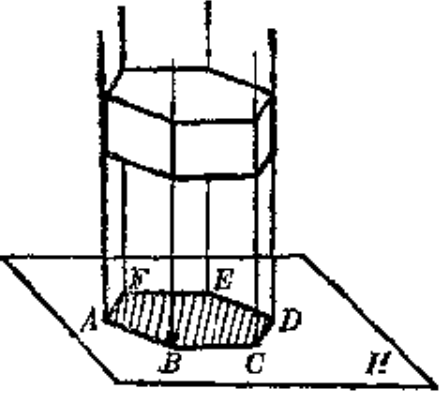
\includegraphics[width=5cm]{../pic/czjh2-ch8-xiti29-01.png}
        \caption*{(第 1 题)}
    \end{minipage}
    \qquad
    \begin{minipage}[b]{10cm}
        \centering
        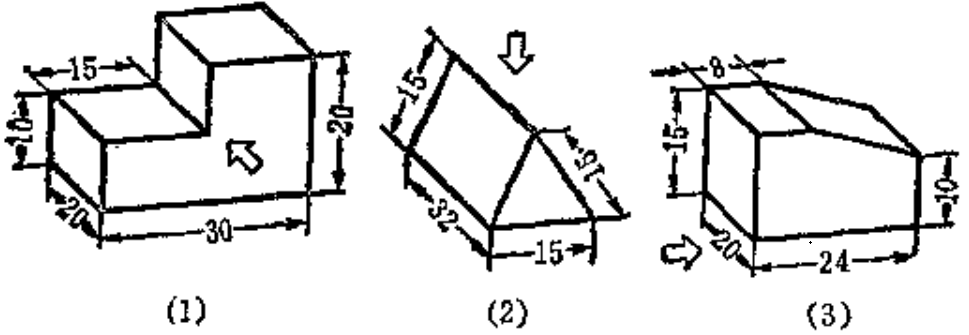
\includegraphics[width=10cm]{../pic/czjh2-ch8-xiti29-02.png}
        \caption*{(第 2 题)}
    \end{minipage}
\end{figure}

\xiaoti{画出所给几何体在指定方向的视图。\footnotemark} % 原题为“下列几何体”,因改变了图片布局。同步修改了题目
\footnotetext{本章习题中的画图题,可用铅笔画,不要求上墨。}


\xiaoti{画出底面半径为 15 mm,高为 30 mm 的圆柱的二视图。}

\begin{figure}[htbp]
    \centering
    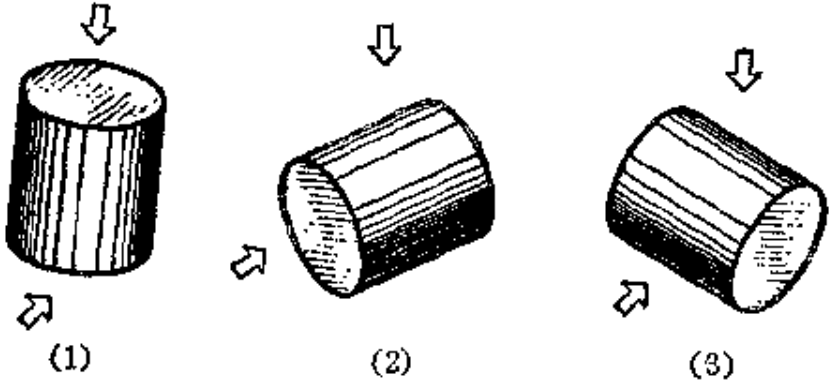
\includegraphics[width=8cm]{../pic/czjh2-ch8-xiti29-03.png}
    \caption*{(第 3 题)}
\end{figure}


\xiaoti{画出下列几何体的二视图。}

\begin{figure}[htbp]
    \centering
    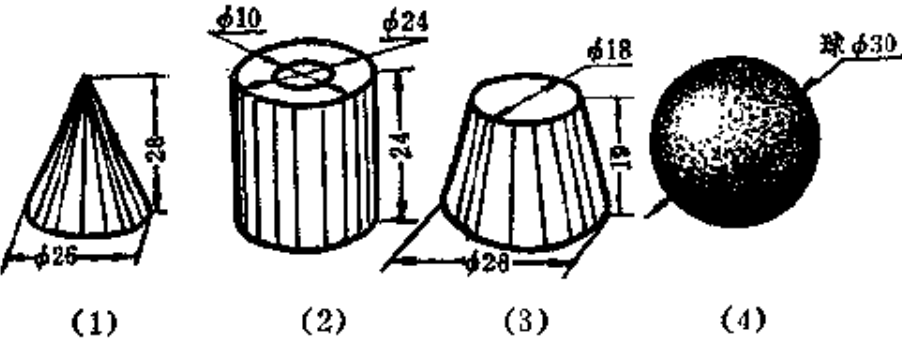
\includegraphics[width=11cm]{../pic/czjh2-ch8-xiti29-04.png}
    \caption*{(第 4 题)}
\end{figure}

\xiaoti{下列几何体的二视图有没有错误(不考虑尺寸)?为什么?如果错了,应该怎样改正?}

\begin{figure}[H]
    \centering
    \begin{minipage}[b]{4cm}
        \centering
        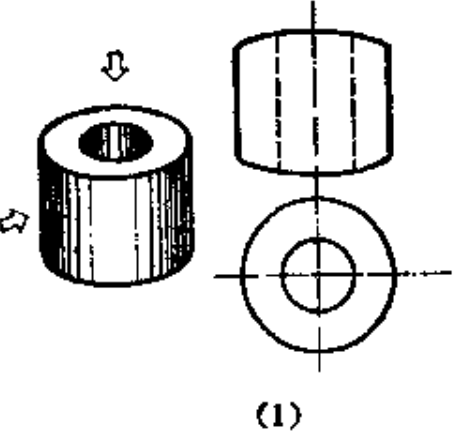
\includegraphics[width=3.5cm]{../pic/czjh2-ch8-xiti29-05-1.png}
    \end{minipage}
    \qquad
    \begin{minipage}[b]{4cm}
        \centering
        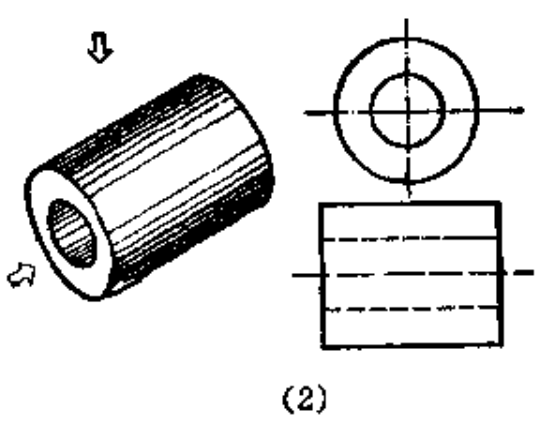
\includegraphics[width=3.8cm]{../pic/czjh2-ch8-xiti29-05-2.png}
    \end{minipage}
    \qquad
    \begin{minipage}[b]{4cm}
        \centering
        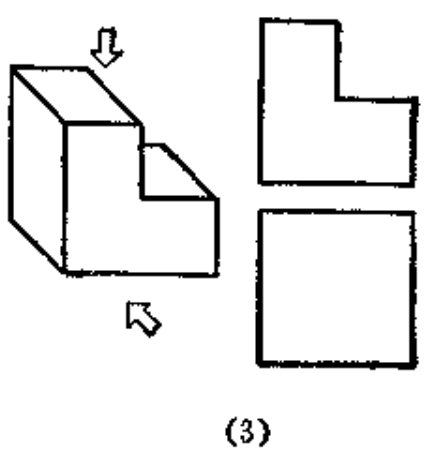
\includegraphics[width=3.3cm]{../pic/czjh2-ch8-xiti29-05-3.png}
    \end{minipage}
\end{figure} % 为了让 1、2、3 小图显示前一页,所以成两个 figure,同时指定属性 [H]

\begin{figure}[H]
    \centering
    \begin{minipage}[b]{4cm}
        \centering
        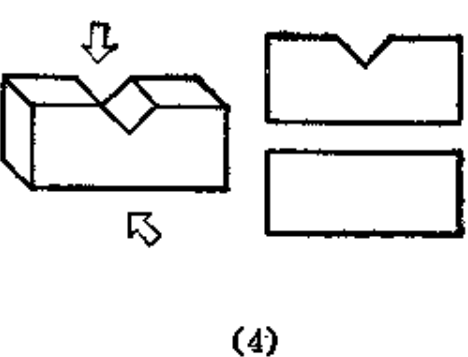
\includegraphics[width=3.8cm]{../pic/czjh2-ch8-xiti29-05-4.png}
    \end{minipage}
    \qquad
    \begin{minipage}[b]{4cm}
        \centering
        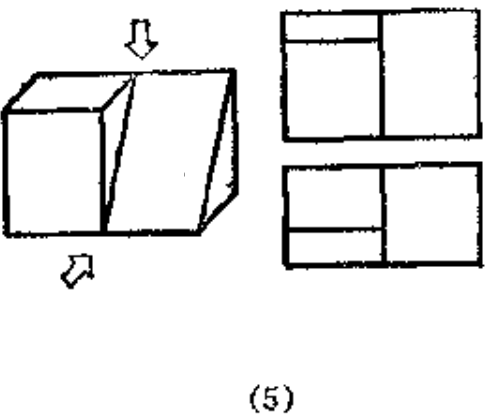
\includegraphics[width=3.5cm]{../pic/czjh2-ch8-xiti29-05-5.png}
    \end{minipage}
    \qquad
    \begin{minipage}[b]{4cm}
        \centering
        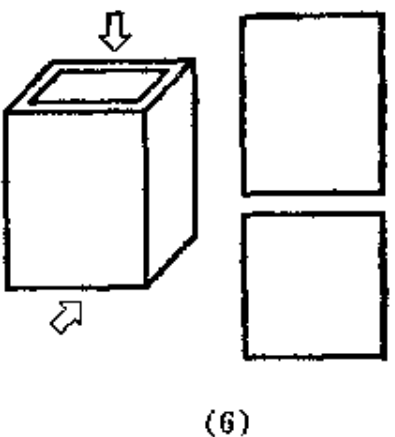
\includegraphics[width=2.8cm]{../pic/czjh2-ch8-xiti29-05-6.png}
    \end{minipage}
    \caption*{(第 5 题)}
\end{figure}

\end{xiaotis}



\subsection{三视图}\label{subsec:czjh2-8-3}

\subsubsection{三视图的概念}

\begin{wrapfigure}[11]{r}{6cm}
    \centering
    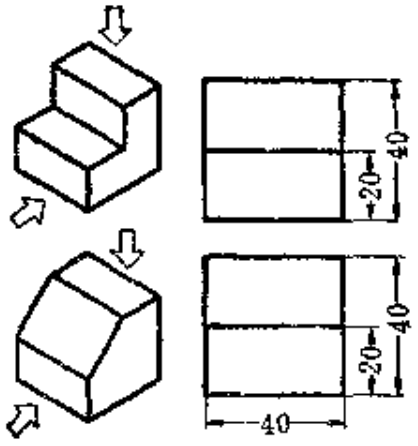
\includegraphics[width=5cm]{../pic/czjh2-ch8-12.png}
    \caption{}\label{fig:czjh2-8-12}
\end{wrapfigure}

有两个大小一样的正方体,棱长为 40 mm,分别切去一块,如图 \ref{fig:czjh2-8-12} 所示。
如果根据指定的方向画它们的二视图,两个几何体的二视图是完全一样的。
这就产生了一个问题,工人根据这样一张二视图的图纸,制造出哪个零件才算合格呢?
可见,对于一些比较复杂的几何体,当用二视图不能反映它的形状和大小时,
往往需要画三个视图或者更多的视图。这里我们只介绍三视图。

如图 \ref{fig:czjh2-8-13},三视图是一个几何体在三个互相垂直的投影面上同时进行正投影所得的三个视图。

除了在正面投影面 $V$ 和水平投影面 $H$ 上的视图外,还增加了在侧面投影面 $W$ 上的视图。
物体在侧面投影面 $W$ 上的视图称为\zhongdian{左视图}。
主视图、俯视图和左视图统称为\zhongdian{三视图}。

\begin{figure}[htbp]
    \centering
    \begin{minipage}[b]{7cm}
        \centering
        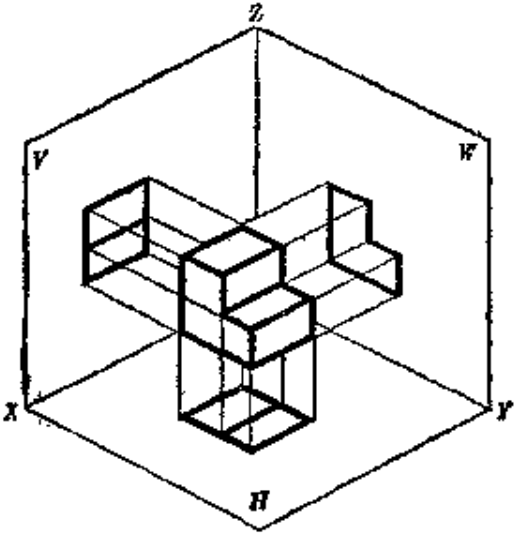
\includegraphics[width=6cm]{../pic/czjh2-ch8-13.png}
        \caption{}\label{fig:czjh2-8-13}
    \end{minipage}
    \begin{minipage}[b]{7cm}
        \centering
        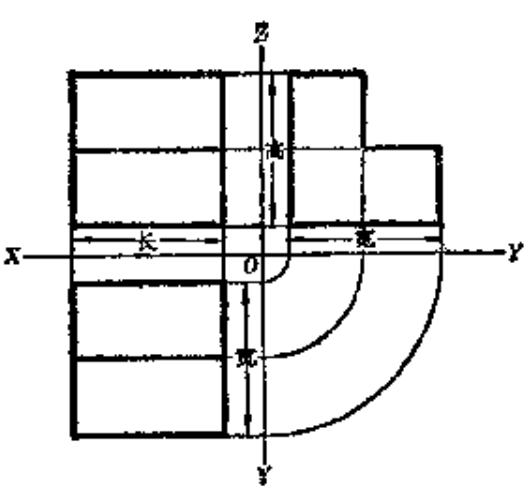
\includegraphics[width=6cm]{../pic/czjh2-ch8-14.png}
        \caption{}\label{fig:czjh2-8-14}
    \end{minipage}
\end{figure}

将几何体拿走后,把投影面 $H$ 向下转 $90^\circ$,投影面 $W$ 向后转 $90^\circ$,
使三个投影面摊平,三个视图就在同一个平面上,如图 \ref{fig:czjh2-8-14}。

三视图的位置是,俯视图在主视图的下面,左视图在主视图的右面。
主视图反映出物体的长和高,俯视图反映出物体的长和宽,左视图反映出物体的高和宽。

因此,三视图的画法规则可以归结为

\begin{center}
    \framebox{\zhongdian{长对正,宽相等,高平齐。}}
\end{center}


\subsubsection{三视图的画法}

我们以图 \ref{fig:czjh2-8-15} (a) 中的物体为例,说明三视图的画法,画图步骤如下:

\begin{figure}[htbp]
    \centering
    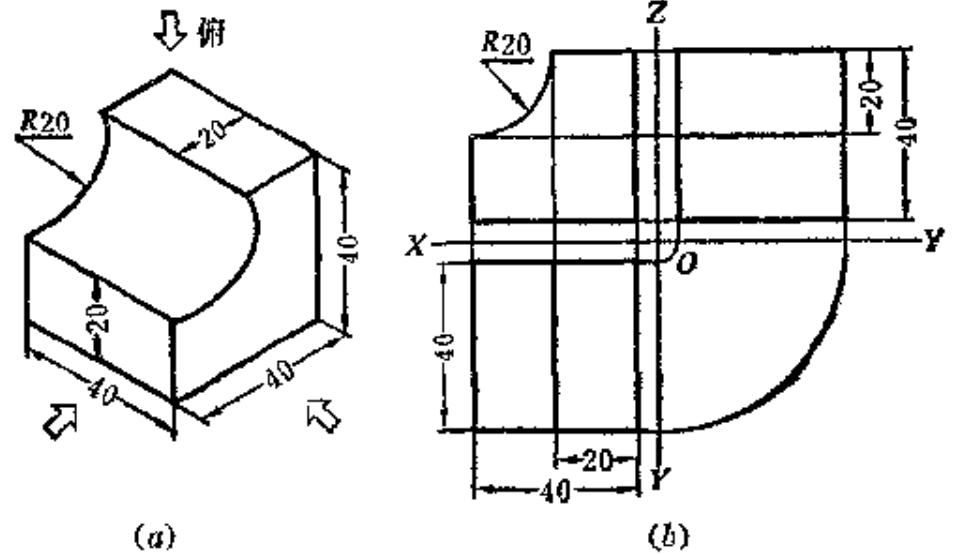
\includegraphics[width=11cm]{../pic/czjh2-ch8-15.png}
    \caption{}\label{fig:czjh2-8-15}
\end{figure}

(1)先画辅助轴线 $XY$、$YZ$ (图画好后可擦掉);

(2)确定主视图的位置,画出主视图;

(3)根据“长对正”与物体的宽度画出俯视图;

(4)再根据“高平齐”与“宽相等”画出左视图(宽度,可通过以点 $O$ 为中心的旋转画出);

(5)标注尺寸,擦去不必要的辅助线。

为了正确表达零件的内外形状,使图面清楚易读,绘图中使用的图线,即线型,应符合统一标准:
轮廓线用粗实线,看不见部分的轮廓线用虚线,尺寸线、尺寸界线用细实线,对称轴线用点划线,
等等(见本章\hyperref[sec:czjh2-8-fulu]{附录})。


\begin{lianxi}

\xiaoti{找出与下列几何体对应的三视图,在三视图下面的括号中填上对应的数码。}

\begin{figure}[H]
    \centering
    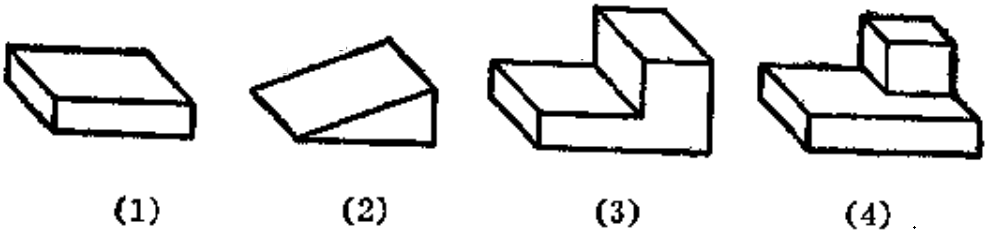
\includegraphics[width=11cm]{../pic/czjh2-ch8-subsec3-lx-01-1.png}
\end{figure}

\begin{figure}[H]
    \centering
    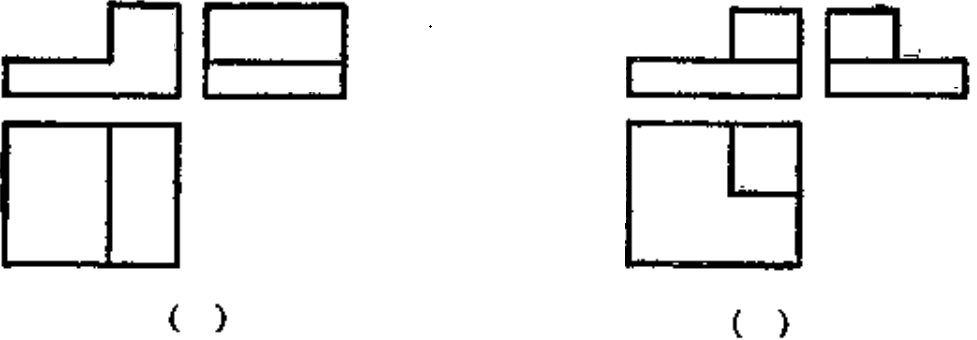
\includegraphics[width=10cm]{../pic/czjh2-ch8-subsec3-lx-01-2.png}
\end{figure}

\begin{figure}[H]
    \centering
    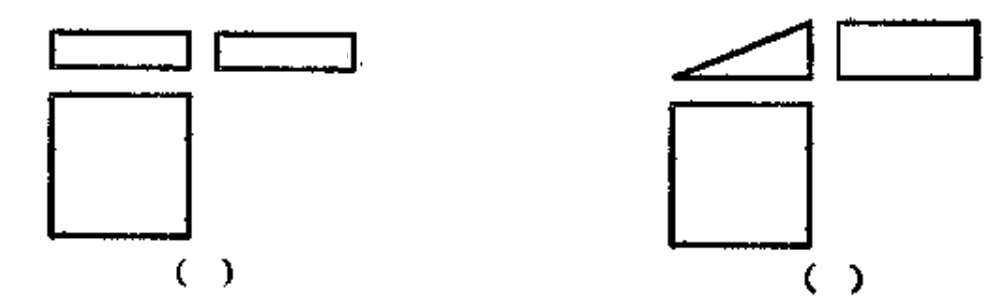
\includegraphics[width=10cm]{../pic/czjh2-ch8-subsec3-lx-01-3.png}
    \caption*{(第 1 题)}
\end{figure}

\xiaoti{添线补全下列三视图。}

\begin{figure}[htbp]
    \centering
    \begin{minipage}[b]{7cm}
        \centering
        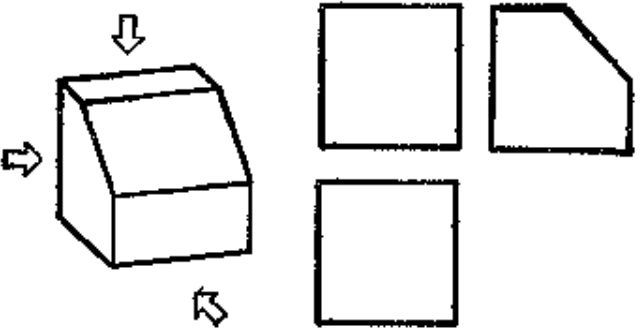
\includegraphics[width=6.8cm]{../pic/czjh2-ch8-subsec3-lx-02-1.png}
        \caption*{(1)}
    \end{minipage}
    \qquad
    \begin{minipage}[b]{7cm}
        \centering
        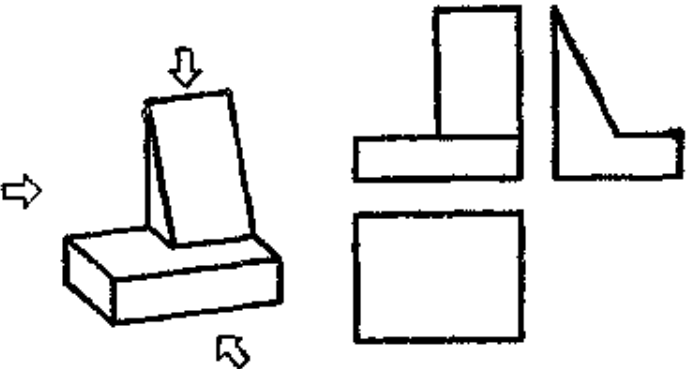
\includegraphics[width=6.8cm]{../pic/czjh2-ch8-subsec3-lx-02-2.png}
        \caption*{(2)}
    \end{minipage}
    \caption*{(第 2 题)}
\end{figure}


\xiaoti{画出下列几何体的三视图。}

\begin{figure}[htbp]
    \centering
    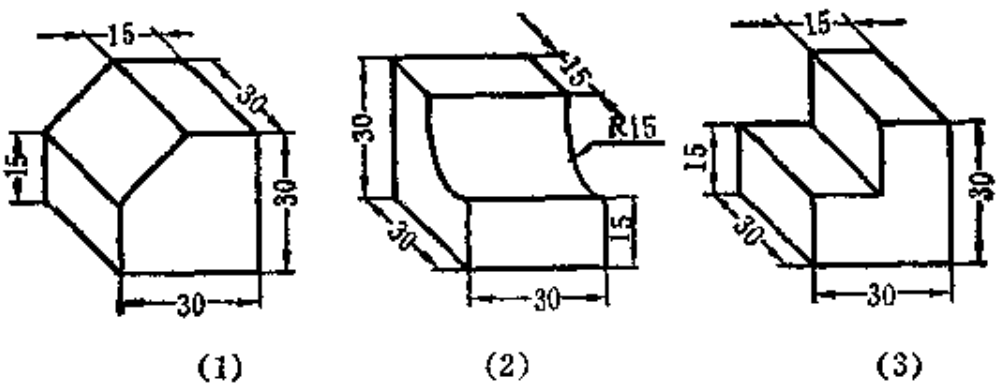
\includegraphics[width=11cm]{../pic/czjh2-ch8-subsec3-lx-03.png}
    \caption*{(第 3 题)}
\end{figure}

\end{lianxi}
\subsection{简单几何体的三视图}\label{subsec:czjh2-8-4}

在生产中所遇到的零件,形状虽然各不相同,但它们一般是由一些简单几何体(柱体、锥体、台体和球体等)组合或切割而成的。
因此熟悉简单几何体的视图是非常必要的,同时这些视图又是工程、机械等制图、识图的基础。
前面已学了一部分简单几何体的视图,这里再介绍棱柱、棱锥、棱台的三视图。


\subsubsection{棱柱的三视图}

画简单体的三视图,一般先画底。以正六棱柱的三视图为例,如果正六棱柱如图 \ref{fig:czjh2-8-16} (a) 这样放置,
那么应该先画俯视图,然后再画其他的视图。

具体画法同前面的三视图画法类似,同学们可按图 \ref{fig:czjh2-8-16} (b)、(c)、(d) 一步步自行分析。
描好轮廓线后,擦去不必要的辅助线,再标注尺寸(图 \ref{fig:czjh2-8-16} (e)),这样,一张图才算完成。

\begin{figure}[htbp]
    \centering
    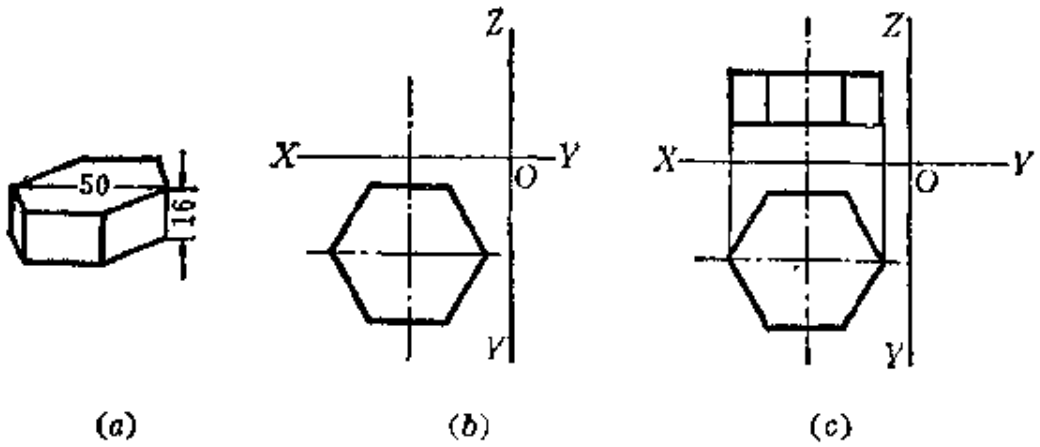
\includegraphics[width=12cm]{../pic/czjh2-ch8-16-1.png}
    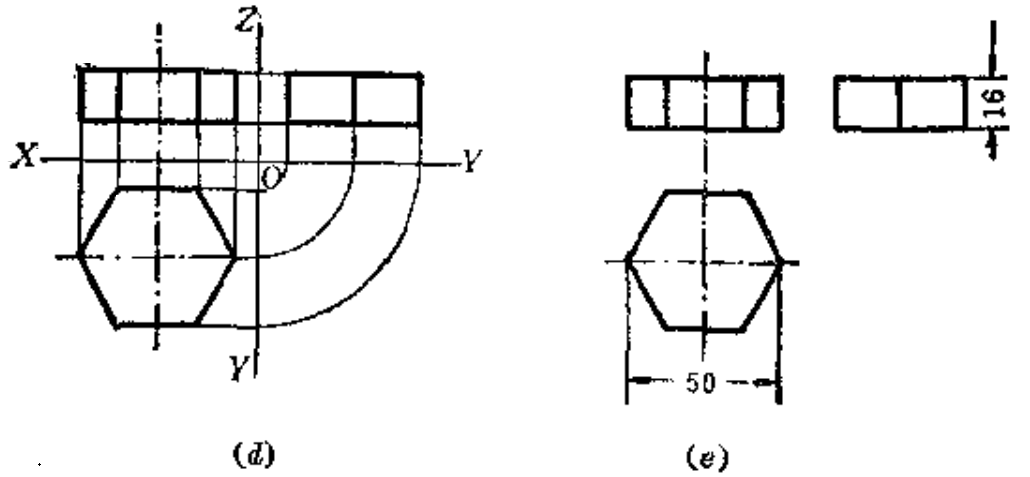
\includegraphics[width=12cm]{../pic/czjh2-ch8-16-2.png}
    \caption{}\label{fig:czjh2-8-16}
\end{figure}

如果正六棱柱如图 \ref{fig:czjh2-8-17} 这样放置,这时画三视图应先画主视图,然后再画其他视图,具体画法与上面一样。

\begin{figure}[htbp]
    \centering
    \begin{minipage}[b]{4cm}
        \centering
        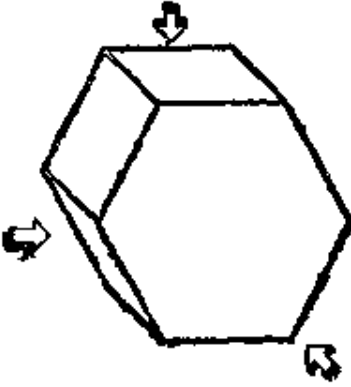
\includegraphics[width=3.5cm]{../pic/czjh2-ch8-17.png}
        \caption{}\label{fig:czjh2-8-17}
    \end{minipage}
    \qquad
    \begin{minipage}[b]{10cm}
        \centering
        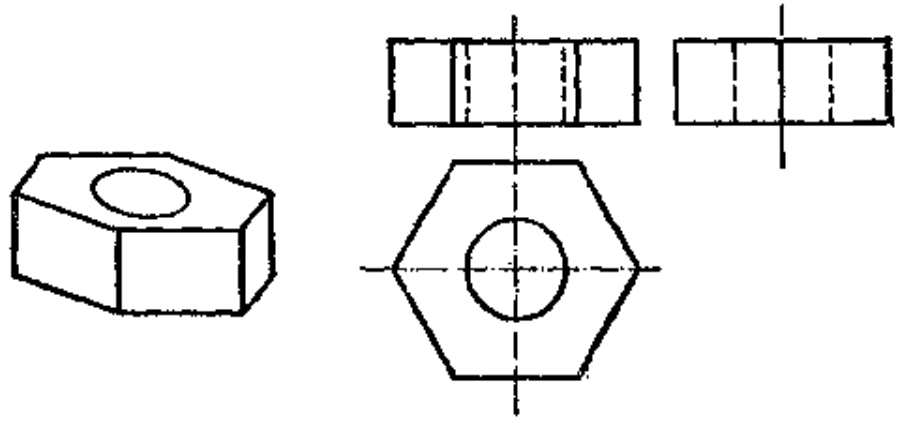
\includegraphics[width=9cm]{../pic/czjh2-ch8-18.png}
        \caption{}\label{fig:czjh2-8-18}
    \end{minipage}
\end{figure}

六角螺母毛坯的三视图,可以看作正六棱柱和圆柱的两个三视图的组合,如图 \ref{fig:czjh2-8-18}。
因为孔的轮廓线是看不见的,所以在主视图与左视图上都要画虚线。


\subsubsection{棱锥、棱台的三视图}

棱锥与棱台的视图画法与棱柱的视图画法是一样的,也是先画底的视图,然后很据三视图规律画出其他的视图。
这里的画法请同学们自行分析。为了便于同学们考虑,图中的辅助线都保留着。

底面边长为 30 mm、高为 30 mm 的正三棱锥的三视图,如图 \ref{fig:czjh2-8-19} 所示。

\begin{figure}[H]%[htbp]
    \centering
    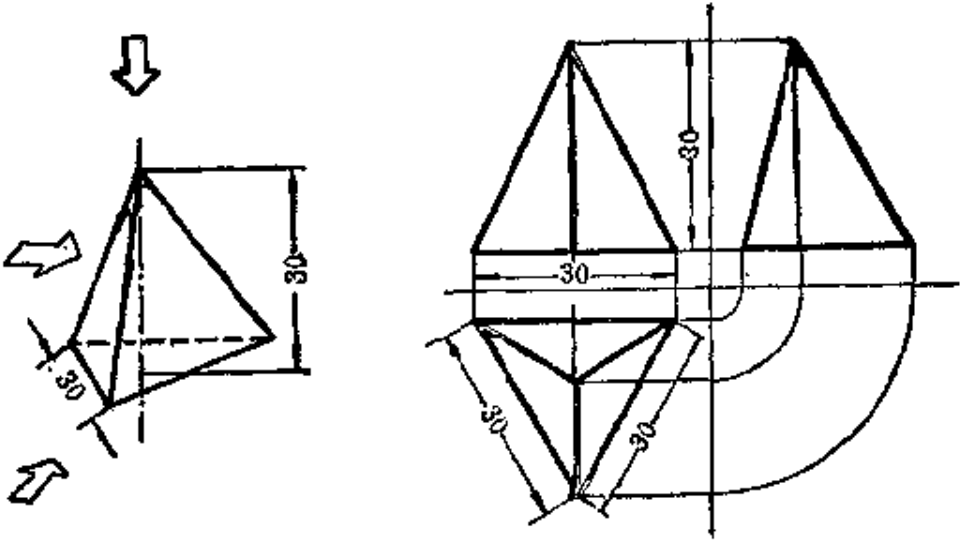
\includegraphics[width=12cm]{../pic/czjh2-ch8-19.png}
    \caption{}\label{fig:czjh2-8-19}
\end{figure}

上底面边长为 20 mm,下底面边长为 40 mm,高为 30 mm 的正四棱台的三视图,如图 \ref{fig:czjh2-8-20} 所示。

\begin{figure}[htbp]
    \centering
    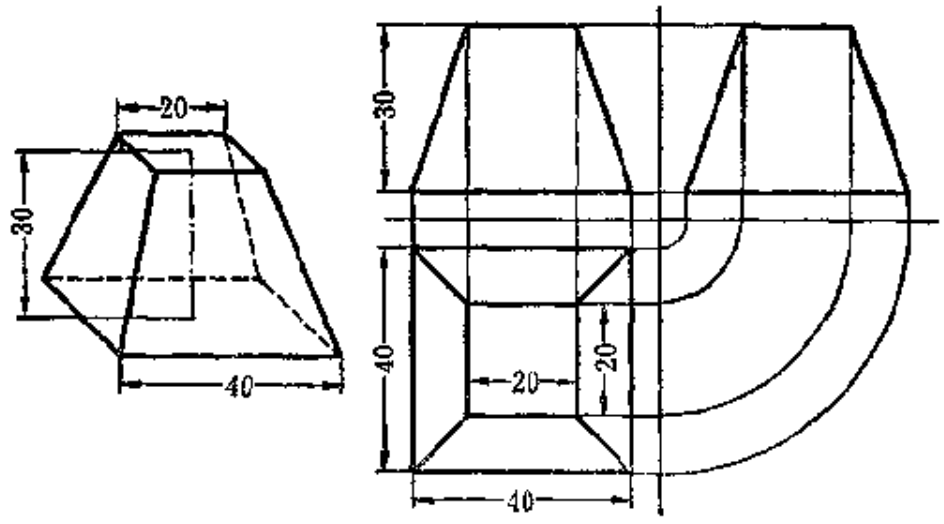
\includegraphics[width=12cm]{../pic/czjh2-ch8-20.png}
    \caption{}\label{fig:czjh2-8-20}
\end{figure}

视图要求简明扼要,通常要使主视图能比较全面地反映物体的特征,而且在不影响表达清楚的前提下,
可以省略左视图或俯视图。如球、圆柱等旋转体在图纸中常用一个视图来表示(如图 \ref{fig:czjh2-8-21} (a)、(b));
棱柱、棱锥、棱台等几何体,常用二视图来表示。
当然也有些复杂的零件用三视图还不能够清楚地表示出来,需要用其他的视图加以补充,这里不再详细说明了。

\begin{figure}[htbp]
    \centering
    \begin{minipage}[b]{10cm}
        \centering
        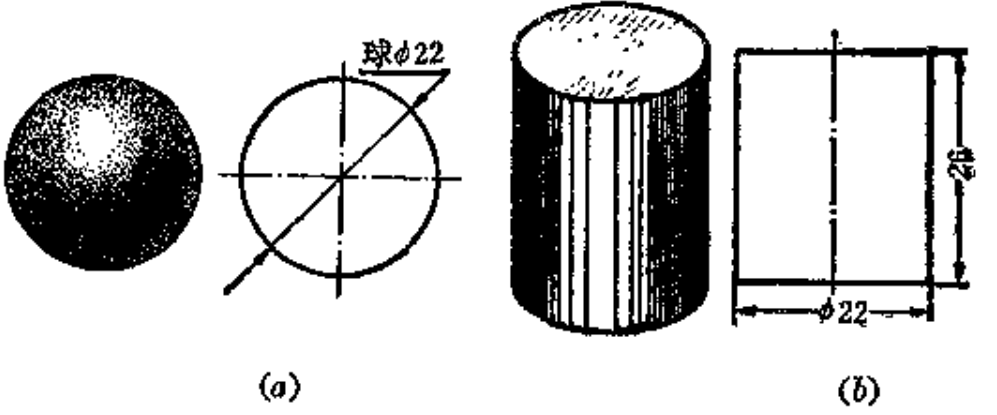
\includegraphics[width=10cm]{../pic/czjh2-ch8-21.png}
        \caption{}\label{fig:czjh2-8-21}
    \end{minipage}
    \qquad
    \begin{minipage}[b]{4cm}
        \centering
        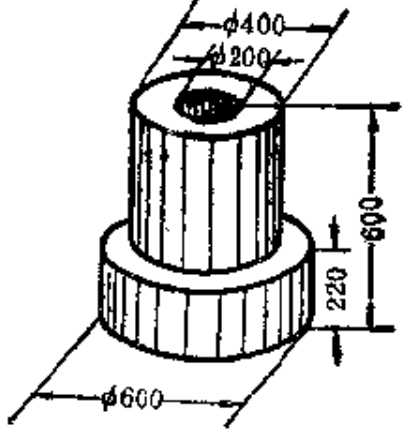
\includegraphics[width=4cm]{../pic/czjh2-ch8-subsec4-lx-01.png}
        \caption*{(第 1 题)}
    \end{minipage}
\end{figure}

\begin{lianxi}

\xiaoti{如果一个零件的尺寸非常大(或者非常小),那么画视图时怎么办?
    试画出一个铸件的三视图,尺寸如图(铸件上面是一个圆柱,下面也是一个圆柱,
    中间挖去一个直径为 200 mm 的圆柱,直通到底)。
    (提示:用适当的比例尺画图,尺寸仍注原件实际尺寸。)
}

\xiaoti{添线补全下列三视图。}

\begin{figure}[htbp]
    \centering
    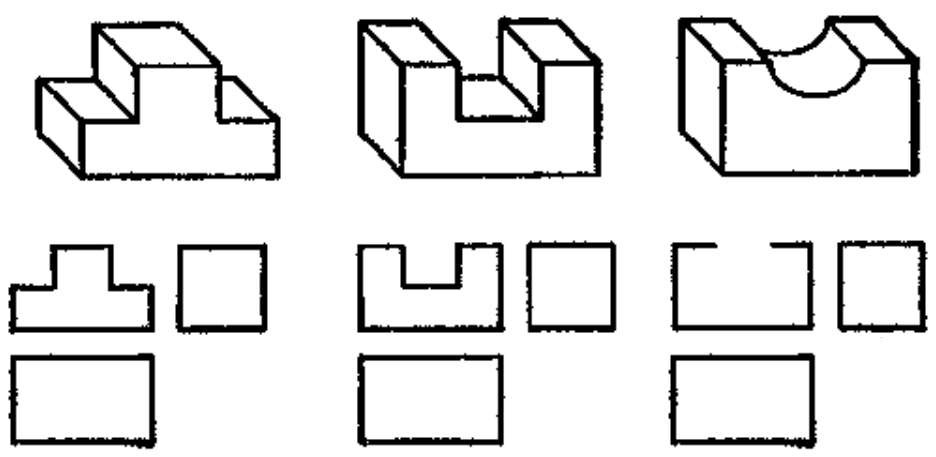
\includegraphics[width=11cm]{../pic/czjh2-ch8-subsec4-lx-02.png}
    \caption*{(第 2 题)}
\end{figure}

\xiaoti{找出下列直观图对应的三视图,在括号中填上对应的数码。}

\begin{figure}[htbp]
    \centering
    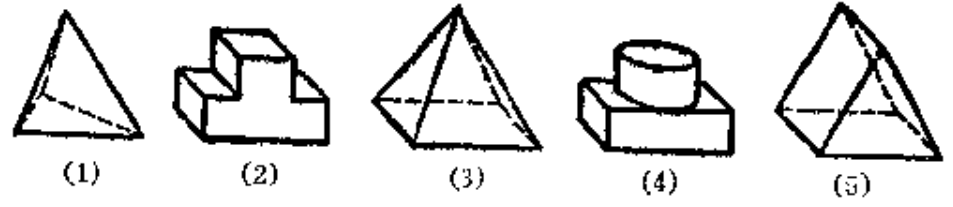
\includegraphics[width=11cm]{../pic/czjh2-ch8-subsec4-lx-03-1.png}
    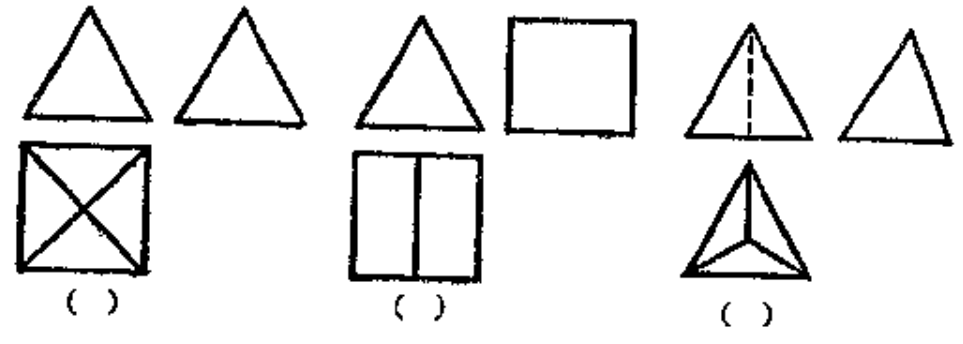
\includegraphics[width=11cm]{../pic/czjh2-ch8-subsec4-lx-03-2.png}
    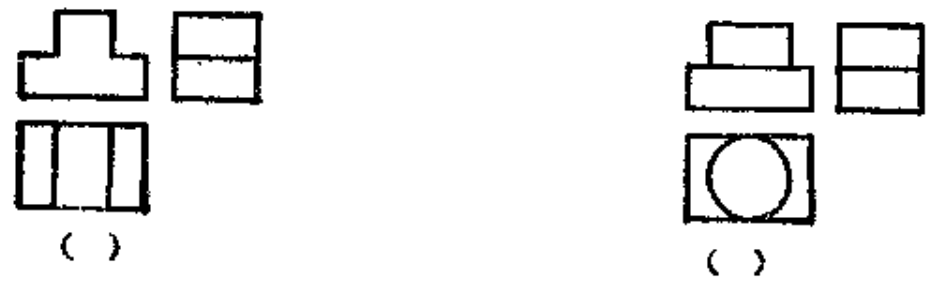
\includegraphics[width=11cm]{../pic/czjh2-ch8-subsec4-lx-03-3.png}
    \caption*{(第 3 题)}
\end{figure}

\end{lianxi}


\newpage % 为了让 xiti30 中的图片显示得更合理
\xiti
\begin{xiaotis}

\xiaoti{画出下列几何体的视图(可以省略某些视图)。}

\begin{figure}[htbp]
    \centering
    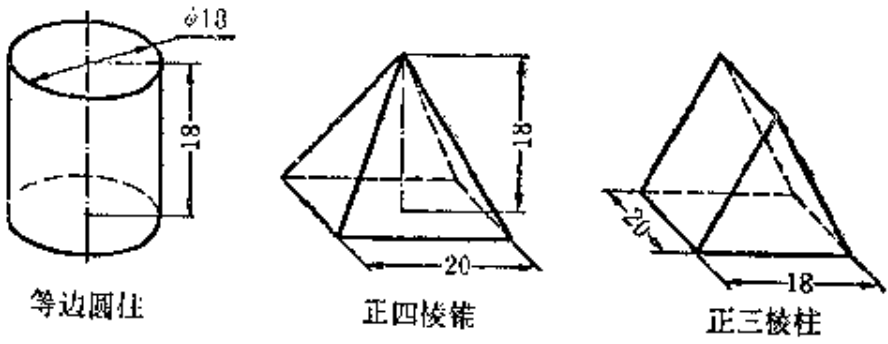
\includegraphics[width=11cm]{../pic/czjh2-ch8-xiti30-01-1.png}
    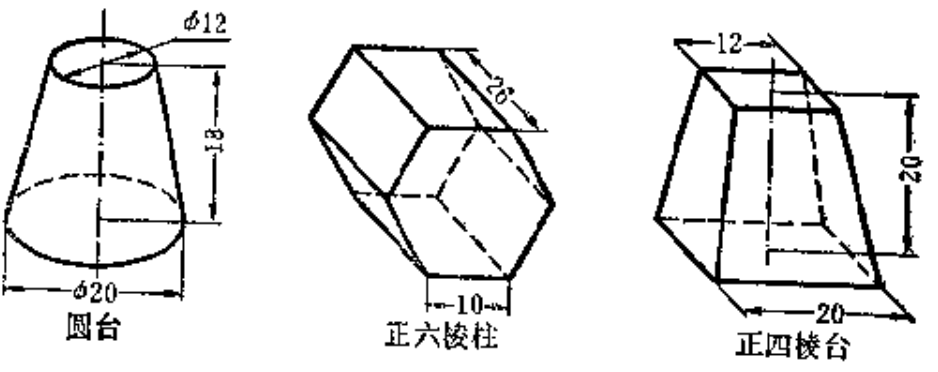
\includegraphics[width=11cm]{../pic/czjh2-ch8-xiti30-01-2.png}
    \includegraphics[width=11cm]{../pic/czjh2-ch8-xiti30-01-3.png}
    \caption*{(第 1 题)}
\end{figure}


\xiaoti{以比例尺 $1.5:1$ 画出下列零件的三视图(提示:比例尺 $1.5:1$ 就是放大成原来的 1.5 倍)。}

\begin{figure}[H]%[htbp]
    \centering
    \includegraphics[width=11cm]{../pic/czjh2-ch8-xiti30-02.png}
    \caption*{(第 2 题)}
\end{figure}

\xiaoti{下列视图有没有错误?为什么?错的如何改正?}

\begin{figure}[htbp]
    \centering
    \includegraphics[width=11cm]{../pic/czjh2-ch8-xiti30-03.png}
    \caption*{(第 3 题)}
\end{figure}

\end{xiaotis}



\xiaojie

一、视图是利用正投影的原理画出的。
正投影的概念是从日常生活中的“影子”加以科学的抽象而得出的。
正投影与光线下物体的“影子”是有区别的,它不是黑的阴影,而是通过规定的线型来表现的,
无论是看得见,或看不见的轮廓线,都要在图上反映出来。
如图 \ref{fig:czjh2-8-22},左图是一般的“影子”,右图是正投影。

在阳光下射线与投影面垂直是很少见的,但正投影概念里投射线与投影面是垂直的。


二、平面形的正投影是画简单几何体视图的基础,平面形的正投影规律是:
平行形不变,倾斜形改变,垂直成线段。

\begin{figure}[htbp]
    \centering
    \includegraphics[width=11cm]{../pic/czjh2-ch8-22.png}
    \caption{}\label{fig:czjh2-8-22}
\end{figure}


三、一些形状复杂的物体可以看成是由简单体切割和组合而成的,掌握了简单体的画法规则后,
就容易掌握这些复杂形体的画法规则。

二视图是学习三视图的基础。对于三视图要注意:长对正,宽相等,高平齐。


四、画视图时,要注意正确运用线型,正确标注尺寸,同时要根据比例尺画图。



\nonumsection{附录}\mylabel{sec:czjh2-8-fulu}
为了清晰、正确地表示视图的轮廓与大小,图纸上所用的线型与尺寸标注,
有统一的标准,现将有关部分简单介绍如下:

\subsubsection{视图中的线型}

\begingroup
\newcommand{\xianxing}[1][]{\tikz \draw[#1] (0,0) -- (3,0);}
\begin{tblr}{hlines,vlines,
    rows={m, rowsep+=3pt}
}
    线型 & 画法 & 主要用途 & 线型粗细标准 \\
    粗实线 & \xianxing[solid, line width=.9mm] & 可见轮廓线 & {粗细为 $b$ \\ $b = 0.1 \text{~} 1.2$ mm} \\
    虚线   & \xianxing[dash pattern=on 15pt off 4pt, line width=.5mm] & 不可见轮廓线 & $\exdfrac{b}{2}$ 左右 \\
    细实线 & \xianxing[solid, line width=.3mm] & 尺寸线、尺寸界线 & $\exdfrac{b}{3}$ 或更细 \\
    点划线 & \xianxing[dash pattern=on 15pt off 3pt on 1pt off 3pt, line width=.3mm] & 轴线和中心线 & $\exdfrac{b}{3}$ 或更细
\end{tblr}
\endgroup

\subsubsection{尺寸注法}

每注一个尺寸时,都要包括下列四个要素:尺寸界线、尺寸线、箭头和尺寸数字,如图 \ref{fig:czjh2-8-23}。

视图上所标注的尺寸是物体的真实大小,与绘图采用的比例尺无关,不标明单位时,是指 mm 。
长度仅用数字表示,
圆的半径在数字前加“$R$”,
圆的直径在数字前加“$\phi$”,
球的直径在数字前加“\mbox{球 $\phi$}”表示。

(1)线段的尺寸注法

尺寸线必须与所注的轮廓线段平行,尺寸界线垂直于被标注的线段。
水平尺寸数字从左到右,铅直尺寸数字从下到上,如图 \ref{fig:czjh2-8-23} 。

\begin{figure}[htbp]
    \centering
    \begin{minipage}[b]{6cm}
        \centering
        \includegraphics[width=6cm]{../pic/czjh2-ch8-23.png}
        \caption{}\label{fig:czjh2-8-23}
    \end{minipage}
    \qquad
    \begin{minipage}[b]{9cm}
        \centering
        \includegraphics[width=9cm]{../pic/czjh2-ch8-24.png}
        \caption{}\label{fig:czjh2-8-24}
    \end{minipage}
\end{figure}

(2)圆与圆弧的尺寸注法

几种注法如图 \ref{fig:czjh2-8-24} 所示。



